\chapter{SLAM系统设计} \label{System Overview}
本章节主要介绍SLAM的概念和原理、一个基本SLAM系统的框架、两个优秀的开源SLAM框架和地图融合算法。

\section{SLAM系统}
同时定位与建图(SLAM,simultaneous localization and mapping)技术,其希望是机器人在对环境和自身所处在环境中的位置未知的情况下,在反复的运动过程中不断观测到的地图特征完成自身位置的定位和姿态的确定,之后再根据自身位置对环境构建增量式的地图,从而达到同时定位与建图的目的。


\subsection{SLAM的分类} \label{3.1.1}
SLAM主要分为视觉SLAM、激光SLAM、融合SLAM和新颖SLAM。


对于视觉SLAM,即用相机完成同时定位与建图的任务。由于相机造价相对较低、电量消耗相对较少、能够获取环境的大量信息,因此相机成为了完成定位与建图任务常用的传感器。视觉SLAM主要有五个步骤,传感器信息读取、视觉里程计(Visual Odometry)、后端优化(Optimization)、回环检测(Loop Closing)、建图(Mapping)[6] 。对于静态、刚体、光照变化不明显、且没有过多人为干扰的场景,视觉SLAM技术已经十分成熟。当前比较好的方案有ORB-SLAM;其在对特征点的描述上做了很大创新,相比于SIFT(尺度不变特征变换,Scale-invariant feature transform)的大计算量和对GPU的特殊需求、FAST关键点描述没有描述子的缺点,ORB改进了FAST的检测子,为其增加了方向性,并且采用了二进制描述子BRIEF(Binary Robust Independent Elementary Feature)[5] 。


对于激光SLAM,主要有两种传感器,单线束激光雷达和多线束激光雷达;单线束激光雷达即2D雷达,2D激光雷达的扫描范围比较单一,角度有限,因此比较适合仅平面运动的机器人的定位与建图,对应的经典算法如GMapping;多线束雷达即3D雷达,其获取的信息包含距离和角度,能够还原出目标的三维点云,且不受光照影响,缺点是造价比较昂贵且易受不良天气影响[7] ,对应的经典算法如谷歌提出的Cartographer。


对于融合SLAM,常见的有视觉和惯性的融合,即相机+IMU(inertial measurement unit,惯性测量单元,包含加速度计和角加速度计)等的多传感器融合;IMU的工作原理是对加速度的积分、初始速度和起始位置进行混合运算,得到运动轨迹和位姿。但是其容易产生漂移(Drift),并且这种累积误差会随时间增加[8] 。


对于VIO(视觉惯性里程计),即上文提到的由相机和惯性测量单元组成的融合传感器,根据融合的框架可以分为松耦合和紧耦合两种。松耦合中对相机关键帧数据的视觉运动估计和对IMU测量数据的运动估计是两个独立的模块,计算时互不干涉;计算完成后将其轨迹结果按一定的方法进行融合。紧耦合则是共同使用相机视觉数据和惯导运动估计数据,共同完成对一组变量的估计;因此其算法更加复杂,且传感器之间的噪声也会相互影响,但是具有更好的效果,也是目前阶段研究的重点方向。这方向上好的方案有VINS-fusion[9]。


对于新颖SLAM,比如语义SLAM;使用神经网络的语义分割、目标检测方法,从图像到位姿,使用其语义分割的结果来完成点云地图的建立和场景识别。语义SLAM能够探测出图像中的各个物体,并且能得到在图像中的位置,可以节省传统的人工标定物品的成本,方便机器人的自主理解能力和简便的人机交互[11] 。


\subsection{成像原理及相机参数} \label{3.1.2}
在各种SLAM中,视觉SLAM由于其传感器(光学相机)造价较低的原因,成为了SLAM中最常用的方式,要了解使用相机的视觉SLAM的原理,首先需要了解相机的成像原理及其参数。

如图\ref{fig4},可以用小孔成像的原理简单地解释针孔相机的模型:
\begin{figure}[!ht]
	\centering
	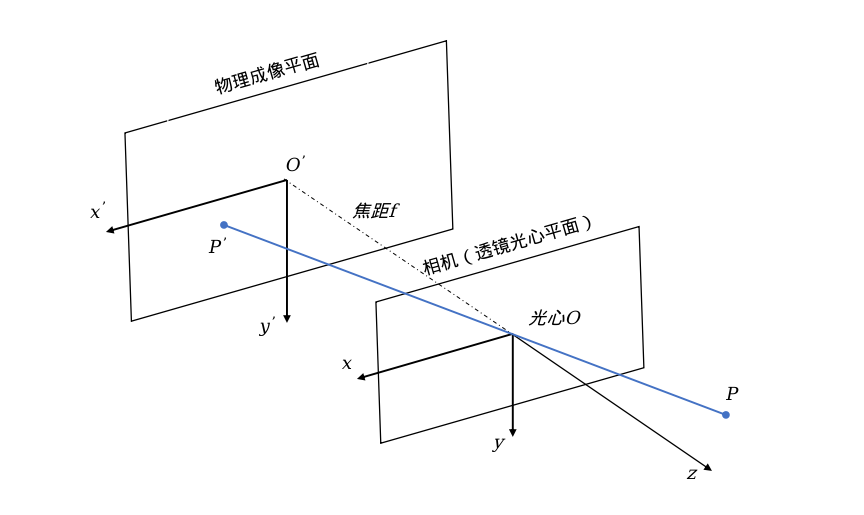
\includegraphics[width=0.6\textwidth]{camera.png}
	\caption{针孔相机模型} 
	\label{fig4}
\end{figure}

$Oxy$平面为相机光心(垂直主光轴)所在的平面,称其为相机平面,对应的$O-x-y-z$坐标系即为相机坐标系;$O'x'y'$平面为物理成像平面,$\bar{OO'}$的长度为焦距$f$;在现实世界中有一点$P$,设其在相机坐标系下的坐标为$[X, Y, Z]^T$,其经过小孔$O$投影后,在相机坐标系下落在像素平面上的坐标为$[X', Y', Z']^T$。

理论下,小孔成像为倒立的实像,但在实际的相机中,成像被人为旋转,成正立的像,因此不考虑坐标系正负号的影响,由相似三角形关系,有:

$$
\frac{Z}{f}=\frac{X}{X'}=\frac{Y}{Y'}
$$

在此基础上,定义像素坐标系。像素坐标系为二维坐标系,在物理成像平面上;像素坐标系的原点位于图像的左上角,横轴为$u$轴,向右与$x$轴平行,纵轴为$v$轴,向下与$y$轴平行,则可以得到像素坐标与$P'$坐标的关系为:

$$
\begin{cases}
u=\alpha X'+c_x=\alpha f \cfrac{X}{Z}+c_x \\
v=\beta Y' +c_y=\beta f  \cfrac{Y}{Z}+c_y \\
\end{cases}
$$

其中,$\alpha$和$\beta$为横轴和纵轴的缩放倍数,$c_x$为图像横向像素的一半,$c_y$为图像纵向像素的一半。令$f_x=\alpha f$,$f_y=\beta f$,将像素坐标系下的坐标转换为齐次坐标:

$$
\begin{bmatrix}
u\\v\\1
\end{bmatrix}=
\frac{1}{Z}
\begin{bmatrix}
f_x & 0 & c_x\\
0   & f_y & c_y\\
0 & 0 & 1
\end{bmatrix}
\begin{bmatrix}
X\\Y\\Z
\end{bmatrix}=
\frac{1}{Z} \bf{KP}
$$

则得到了相机的内参矩阵(Camera Intrinsics)$\bf{K}$。通常情况下,对于焦距固定的相机(或定焦镜头),其出厂之后内参矩阵是固定的;如果无法从厂家得到相机的内参,可以使用标定的方法获得相机的内参矩阵,常见的标定算法有张正友标定法。

除相机的内参外,还有相机外参(Camera Extrinsics)的定义;相机的外参由其旋转矩阵$\bf{R}$和平移向量$\bf{t}$构成。对于$P$点而言,其在相机坐标系(像素坐标平面)下的坐标应为其在世界坐标系下的坐标根据相机相对于世界坐标系的位姿所变换得到的,相机的位姿即由其外参决定,则世界坐标系下$P$点的坐标$\bf{P_w}$在相机坐标系下的坐标为:

$$
Z
\begin{bmatrix}
u\\v\\1
\end{bmatrix}=
\bf{K(RP_w+t)}
$$

\subsection{视觉SLAM的基本步骤} \label{3.1.3}

经典的视觉SLAM框架如图\ref{fig5}所示:

\begin{figure}[!ht]
	\centering
	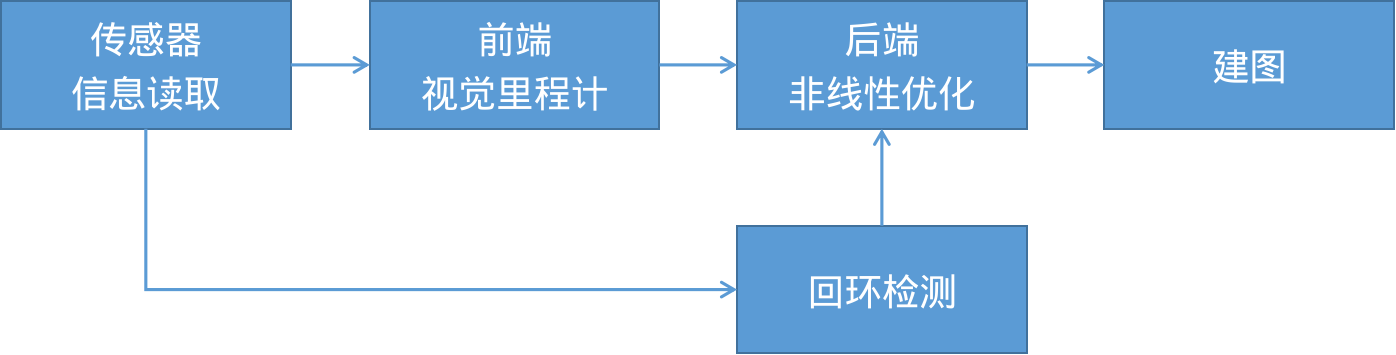
\includegraphics[width=0.6\textwidth]{SLAM.png}
	\caption{经典视觉SLAM框架} 
	\label{fig5}
\end{figure}

经典视觉SLAM流程包括以下基本步骤:
\begin{enumerate}
	\item 
	传感器信息读取。主要为相机图像的读取以及一些预处理步骤,在不同的视觉SLAM算法中,可能还涉及惯性测量元件信息的读取和预处理。
	\item 
	前端视觉里程计(Visual Odometry)。视觉里程计的功能是从相邻的几帧图像之中,根据几何约束,得到相机的运动;并且通过记录地图点(路标)与相机的相对位置,构建局部地图。
	\item 
	后端(非线性)优化(Optimization)。后端主要涉及滤波与非线性优化算法,其目的是减少传感器的误差,完成对运动的相机和周围环境的不确定性的估计。
	\item 
	回环检测(Loop Closure Detection)。回环检测的作用是使机器人能够分辨出当前面临的场景是否曾经来到过,解决位置估计的误差随时间累计,发生漂移的问题;并且消除累计误差,最终得到全局一致的轨迹和地图。
	\item 
	建图(Mapping)。建图即根据前端里程计和后端优化得到的地图点(路标点),构建地图。
\end{enumerate}

% 视觉里程计
视觉里程计是SLAM的关键,其基本完成了同时定位与建图的任务。视觉里程计的实现主要有两种方法:特征点法和直接法。

% 特征点法
特征点法作为很长时间以来视觉里程计的主要方法,其特点是比较稳定,在光照差异大和画面中有动态物体的情况下也能较好地完成任务。特征点法的核心在特征点的提取与匹配;提取即从每帧图像中找到可以代表图像特征的点,辨识度更高的点。

\begin{figure}[!ht]
	\centering
	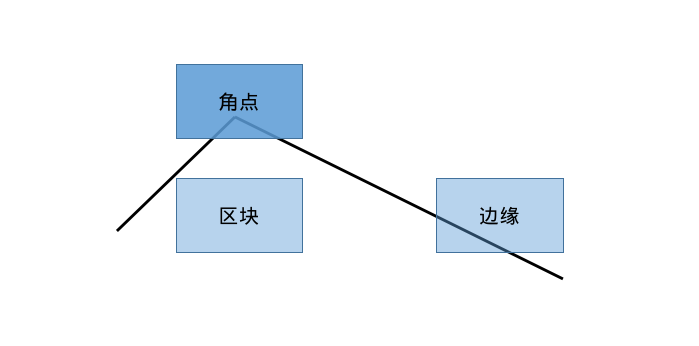
\includegraphics[width=0.6\textwidth]{corner.png}
	\caption{角点、边缘、区块} 
	\label{fig6}
\end{figure}

特征点的一种方法是使用角点。如图\ref{fig6},可以把一张图像中的内容分为角点、边缘、区块三种类型。可以发现,指出某两张图像中出现的统一区块是最难以实现的,因为存在大面积相同的色块,无法确定具体点的匹配;其次是边缘,其具有一定的特征,但沿边缘行进,仍可能出现相同的局部特征,造成误匹配;因此选择其中最具有特征角点作为特征。性能较好、比较稳定的角点有SIFT、SURF,ORB等。

% 对极几何与三角测量
在完成特征点提取与匹配后,根据不同的传感器类型,有不同的得到相机位姿的方法。对于传统的单目相机传感器,可以使用对极几何约束,得到相机的运动,并通过三角测量的方法恢复地图点相对于每时刻相机的位置。

% 直接法
前端视觉里程计的另一种方法是直接法,由光流法演变而来。光流法与特征点法不同,特征点法使用特征点的描述子来完成特征匹配,而光流法可以跟踪特征点的运动,这样就无需进行大量的描述子匹配运算。直接法可以弥补特征点法的一些缺陷。


% 优化
后端优化主要有两种方法,滤波和非线性优化。拓展卡尔曼滤波EKF及其演变出的粒子滤波方法等,在早期的SLAM设计中应用十分广泛。但随着非线性优化方法的普及,现在的SLAM方案多用BA图优化及位姿图优化的方法,并且有可以使用的ceres和g2o库。

% 回环检测
回环检测在判断场景是否曾经来过时,一般用的是词袋模型(Bag of Words),根据图像中是否存在同样的几种相似特征来判断是否在外观上相似。

% 建图
建图根据地图的需求,可以分为用于定位的稀疏地图,用于导航、重建的稠密地图和用于交互的语义地图。按照地图的分类,可以分为拓扑地图和度量地图两种;拓扑地图着重与图节点之间的连通性,而度量地图则能够精确地表示出地图点相对于相机的位置。


\subsection{对极几何约束与三角测量} \label{3.1.4}


\section{ORB-SLAM2}

ORB-SLAM2是由萨拉戈萨大学的Raúl Mur-Artal开发,可以用在单目、双目、RGB-D深度相机的视觉SLAM系统。

\subsection{ORB特征点及描述子} \label{3.2.1}

% 简单介绍 
ORB特征点是上文\ref{3.1.3}提到过的特征点的一种,它的全称是Oriented FAST and Rotated BRIEF;其中,FAST是角点的一种,BRIEF是Binary Robust Independent Elementary Feature,是一种二进制描述子;ORB特征点即由改进的FAST关键点和带旋转的BRIEF描述子组成。

% FAST
FAST角点选取的核心思想是,选取的点和周边像素点亮度差别很大,则该点可能是FAST角点。如图\ref{fig7}所示,对于可能被选取为FAST角点的像素点$p$,其亮度为$I_p$;设置亮度差异的阈值$T$,可以为$0.3I_p$;选取半径为3的圆上的16个点,对应图中的16个深色点,记录各点的像素值$I_i$,如果16个点中有连续$N$各点满足$|I_i-I_p|>T$,则像素点$p$可以被认为是FAST角点,该标准为FAST-N,N一般取9、11、12。

% Oriented FAST



\begin{figure}[!ht]
	\centering
	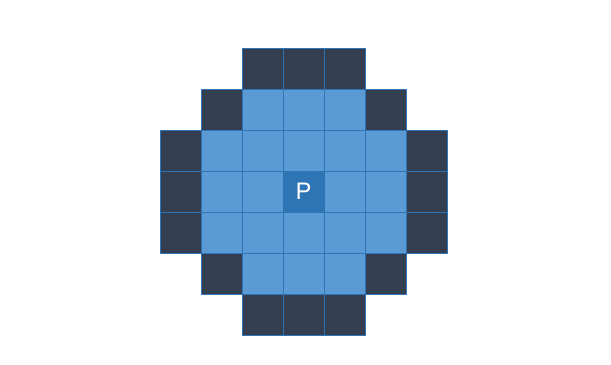
\includegraphics[width=0.5\textwidth]{FAST.png}
	\caption{FAST关键点} 
	\label{fig7}
\end{figure}

\subsection{ORB-SLAM2的主要进程} \label{3.2.2}


\section{CCM-SLAM}

\subsection{CCM-SLAM的结构} \label{3.3.1}
\subsection{Client与Server机制} \label{3.3.2}


\section{多机协同及地图融合方案}

\subsection{算法原理} \label{3.4.1}
\subsection{编程实现} \label{3.4.2}